%% Преамбула TeX-файла

% 1. Стиль и язык
\documentclass[utf8x, 12pt]{G7-32} % Стиль (по умолчанию будет 14pt)

% Остальные стандартные настройки убраны в preamble.inc.tex.
\sloppy

% Настройки стиля ГОСТ 7-32
% Для начала определяем, хотим мы или нет, чтобы рисунки и таблицы нумеровались в пределах раздела, или нам нужна сквозная нумерация.
\EqInChapter % формулы будут нумероваться в пределах раздела
\TableInChapter % таблицы будут нумероваться в пределах раздела
\PicInChapter % рисунки будут нумероваться в пределах раздела
\usepackage{slashbox}

% Добавляем гипертекстовое оглавление в PDF
\usepackage[
bookmarks=true, colorlinks=true, unicode=true,
urlcolor=black,linkcolor=black, anchorcolor=black,
citecolor=black, menucolor=black, filecolor=black,
]{hyperref}

% Изменение начертания шрифта --- после чего выглядит таймсоподобно.
% apt-get install scalable-cyrfonts-tex

\IfFileExists{cyrtimes.sty}
    {
        \usepackage{cyrtimespatched}
    }
    {
        % А если Times нету, то будет CM...
    }

\usepackage{graphicx}   % Пакет для включения рисунков
\usepackage{subfig}

% С такими оно полями оно работает по-умолчанию:
% \RequirePackage[left=20mm,right=10mm,top=20mm,bottom=20mm,headsep=0pt]{geometry}
% Если вас тошнит от поля в 10мм --- увеличивайте до 20-ти, ну и про переплёт не забывайте:
\geometry{right=20mm}
\geometry{left=30mm}


% Пакет Tikz
\usepackage{tikz}
\usetikzlibrary{arrows,positioning,shadows}

% Произвольная нумерация списков.
\usepackage{enumerate}

% ячейки в несколько строчек
\usepackage{multirow}

% itemize внутри tabular
\usepackage{paralist,array}

% Центрирование подписей к плавающим окружениям
\usepackage[justification=centering]{caption}

% Нормальное нижнее подчеркивание
\usepackage{ulem}

% Графики
\usepackage{pgfplots}
\pgfplotsset{compat=1.9}

% Для ссылок в списке использованных источников и возможности их переноса
\usepackage{url}
\def\UrlBreaks{\do\A\do\B\do\C\do\D\do\E\do\F\do\G\do\H\do\I\do\J
	\do\K\do\L\do\M\do\N\do\O\do\P\do\Q\do\R\do\S\do\T\do\U\do\V
	\do\W\do\X\do\Y\do\Z\do\[\do\\\do\]\do\^\do\_\do\`\do\a\do\b
	\do\c\do\d\do\e\do\f\do\g\do\h\do\i\do\j\do\k\do\l\do\m\do\n
	\do\o\do\p\do\q\do\r\do\s\do\t\do\u\do\v\do\w\do\x\do\y\do\z
	\do\.\do\@\do\\\do\/\do\!\do\_\do\|\do\;\do\>\do\]\do\)\do\,
	\do\?\do\'\do+\do\=\do\#}


% Настройки листингов.
\ifPDFTeX
% 8 Листинги

\usepackage{listings}
\usepackage{wrapfig}
% Значения по умолчанию
\lstset{
  basicstyle= \footnotesize,
  breakatwhitespace=true,% разрыв строк только на whitespacce
  breaklines=true,       % переносить длинные строки
%   captionpos=b,          % подписи снизу -- вроде не надо
  inputencoding=koi8-r,
  numbers=left,          % нумерация слева
  numberstyle=\footnotesize,
  showspaces=false,      % показывать пробелы подчеркиваниями -- идиотизм 70-х годов
  showstringspaces=false,
  showtabs=false,        % и табы тоже
  stepnumber=1,
  tabsize=4,              % кому нужны табы по 8 символов?
  frame=single
}

% Стиль для псевдокода: строчки обычно короткие, поэтому размер шрифта побольше
\lstdefinestyle{pseudocode}{
  basicstyle=\small,
  keywordstyle=\color{black}\bfseries\underbar,
  language=Pseudocode,
  numberstyle=\footnotesize,
  commentstyle=\footnotesize\it
}

% Стиль для обычного кода: маленький шрифт
\lstdefinestyle{realcode}{
  basicstyle=\scriptsize,
  numberstyle=\footnotesize
}

% Стиль для коротких кусков обычного кода: средний шрифт
\lstdefinestyle{simplecode}{
  basicstyle=\footnotesize,
  numberstyle=\footnotesize
}

% Стиль для BNF
\lstdefinestyle{grammar}{
  basicstyle=\footnotesize,
  numberstyle=\footnotesize,
  stringstyle=\bfseries\ttfamily,
  language=BNF
}

% Определим свой язык для написания псевдокодов на основе Python
\lstdefinelanguage[]{Pseudocode}[]{Python}{
  morekeywords={each,empty,wait,do},% ключевые слова добавлять сюда
  morecomment=[s]{\{}{\}},% комменты {а-ля Pascal} смотрятся нагляднее
  literate=% а сюда добавлять операторы, которые хотите отображать как мат. символы
    {->}{\ensuremath{$\rightarrow$}~}2%
    {<-}{\ensuremath{$\leftarrow$}~}2%
    {:=}{\ensuremath{$\leftarrow$}~}2%
    {<--}{\ensuremath{$\Longleftarrow$}~}2%
}[keywords,comments]

% Свой язык для задания грамматик в BNF
\lstdefinelanguage[]{BNF}[]{}{
  morekeywords={},
  morecomment=[s]{@}{@},
  morestring=[b]",%
  literate=%
    {->}{\ensuremath{$\rightarrow$}~}2%
    {*}{\ensuremath{$^*$}~}2%
    {+}{\ensuremath{$^+$}~}2%
    {|}{\ensuremath{$|$}~}2%
}[keywords,comments,strings]

% Подписи к листингам на русском языке.
\renewcommand\lstlistingname{\cyr\CYRL\cyri\cyrs\cyrt\cyri\cyrn\cyrg}
\renewcommand\lstlistlistingname{\cyr\CYRL\cyri\cyrs\cyrt\cyri\cyrn\cyrg\cyri}

\else
\usepackage{local-minted}
\fi

% Полезные макросы листингов.
% Любимые команды
\newcommand{\Code}[1]{\textbf{#1}}



\begin{document}

\frontmatter % выключает нумерацию ВСЕГО; здесь начинаются ненумерованные главы: реферат, введение, глоссарий, сокращения и прочее.

% Команды \breakingbeforechapters и \nonbreakingbeforechapters
% управляют разрывом страницы перед главами.
% По-умолчанию страница разрывается.

% \nobreakingbeforechapters
% \breakingbeforechapters

% % Также можно использовать \Referat, как в оригинале
%\begin{abstract}
%	Титульный лист. Эта страница нужна мне, чтобы не сбивалась нумерация страниц
%	\cite{Dh}
%	\cite{Bayer}
%	\cite{Habr1}
%	\cite{Noise_func}
%	\cite{Ulich}

%Это пример каркаса расчётно-пояснительной записки, желательный к использованию в РПЗ проекта по курсу РСОИ.

%Данный опус, как и более новые версии этого документа, можно взять по адресу (\url{https://github.com/rominf/latex-g7-32}).

%Текст в документе носит совершенно абстрактный характер.
%\end{abstract}


\newenvironment{signstabular}[1][1]{
	\renewcommand*{\arraystretch}{#1}
	\tabular
}{
	\endtabular
}




\begin{titlepage}
	\thispagestyle{empty}
	
	\noindent\begin{minipage}{0.05\textwidth}
		
\includegraphics[scale=0.3]{img/bmstu.png}
	\end{minipage}
	\hfill
	\begin{minipage}{0.85\textwidth}\raggedleft
		\begin{center}
			\fontsize{12pt}{0.3\baselineskip}\selectfont \textbf{Министерство науки и высшего образования Российской Федерации \\ Федеральное государственное бюджетное образовательное учреждение \\ высшего образования \\ <<Московский государственный технический университет \\ имени Н.Э. Баумана \\ (национальный исследовательский университет)>> \\ (МГТУ им. Н.Э. Баумана)}
		\end{center}
	\end{minipage}
	
	\begin{center}
		\fontsize{12pt}{0.1\baselineskip}\selectfont
		\noindent\makebox[\linewidth]{\rule{\textwidth}{4pt}} \makebox[\linewidth]{\rule{\textwidth}{1pt}}
	\end{center}
	
	\begin{flushleft}
		\fontsize{12pt}{0.8\baselineskip}\selectfont
		
		ФАКУЛЬТЕТ \uline{
			Информатика и системы управления
			\hfill}
		
		КАФЕДРА \uline{\mbox{\hspace{4mm}}
			Программное обеспечение ЭВМ и информационные технологии
			\hfill}
	\end{flushleft}
	
	\vfill
	
	\begin{center}
		\fontsize{20pt}{\baselineskip}\selectfont
		
		\textbf{РАСЧЕТНО-ПОЯСНИТЕЛЬНАЯ ЗАПИСКА}
		
		\textbf{\textit{К КУРСОВОМУ ПРОЕКТУ}}
		
		\textbf{\textit{НА ТЕМУ:}}
	\end{center}
	
	\begin{center}
		\fontsize{18pt}{0.6cm}\selectfont
		
		Разработка инструмента для построения трёхмерных изображений, ориентированного на микроконтроллеры STM32
		
	\end{center}
	
	\vfill
	
	\begin{table}[h!]
		\fontsize{12pt}{0.7\baselineskip}\selectfont
		\centering
		\begin{signstabular}[0.7]{p{7.25cm} >{\centering\arraybackslash}p{4cm} >{\centering\arraybackslash}p{4cm}}
			Студент группы \uline{ИУ7-53Б} & \uline{\mbox{\hspace*{4cm}}} & \uline{\hfill А.М. Сапожков  \hfill} \\
			& \scriptsize (Подпись, дата) & \scriptsize (И.О. Фамилия)
		\end{signstabular}
		
		\vspace{\baselineskip}
		
		\begin{signstabular}[0.7]{p{7.25cm} >{\centering\arraybackslash}p{4cm} >{\centering\arraybackslash}p{4cm}}
			Руководитель курсовой работы & \uline{\mbox{\hspace*{4cm}}} & \uline{\hfill Ю.В. Строганов \hfill} \\
			& \scriptsize (Подпись, дата) & \scriptsize (И.О. Фамилия)
		\end{signstabular}
		
		% \vspace{\baselineskip}
		
		% \begin{signstabular}[0.7]{p{7.25cm} >{\centering\arraybackslash}p{4cm} >{\centering\arraybackslash}p{4cm}}
			%     Консультант & \uline{\mbox{\hspace*{4cm}}} & \uline{\hfill  \hfill} \\
			%     & \scriptsize (Подпись, дата) & \scriptsize (И.О. Фамилия)
			% \end{signstabular}
	\end{table}
	
	\vfill
	
	\begin{center}
		\normalsize \textit{\textbf{2022} г.}
	\end{center}
\end{titlepage}


\textbf{Титульный лист.}
\newpage

\textbf{Техническое задание.}
\newpage

\tableofcontents

% \Defines % Необходимые определения. Вряд ли понадобться
\begin{description}
	
	%\textbf{test} 
	\item[Рендеринг] процесс получения изображения по двумерной или трёхмерной модели 
	с помощью компьютерной программы.%\cite{Wiki_artifact}
	%\item[Цифровой шум] дефект изображения, вносимый фотосенсорами и электроникой устройств, которые их используют вследствие несовершенства технологий.
	%Цифровой шум заметен на изображении в виде наложенной маски из пикселей случайного цвета и яркости \cite{Wiki_noise}
	
	%\item[Фиксированная пороговая обработка (fixed thresholding)] -обработка пикселя на основе какого-то фиксированного порового значения. В случае если текущее значения пикселя больше этого порогового значения, пиксель закрашивает одним фиксированным цветом, иначе -другим. 
	%\cite{Dh}
	%\item[Интенсивность цвета]  степень отличия хроматического цвета от равного ему по светлоте ахроматического, «глубина» цвета. Два оттенка одного тона могут различаться степенью блёклости. При уменьшении насыщенности каждый хроматический цвет приближается к серому.\cite{Wiki_intens}
	%\item[Ахроматические цвета] оттенки серого (в диапазоне белый — чёрный).\cite{Wiki_achrom}
	%\item[Монохромное изображение] изображение, содержащее свет одного цвета (длины волны), воспринимаемый, как один оттенок (в отличие от цветного изображения, содержащего различные цвета).\cite{Wiki_hrom}
	%\item[Цвета шума]система терминов, приписывающая некоторым видам стационарных шумовых сигналов определённые цвета исходя из аналогии между спектром сигнала произвольной природы.\cite{Wiki_color_noise}
	%\item[Спектральная плотность S(w) стационарного случайного процесса x(t) ] это частотная функция, характеризующая спектральный (частотный) состав процесса, и представляет собой частотную характеристику для средних значений квадратов амплитуд гармоник, на которые может быть разложен случайный процесс.\cite{Wiki_staz}
	%\item[Светлый пиксель] пиксель,код цвета которого более или равен 128 для одноцветной палитры 0-255.
	%\item[Темный пиксель] пиксель,код цвета которого менее  128 для одноцветной палитры 0-255.
	
	
	
\end{description}

%%% Local Variables:
%%% mode: latex
%%% TeX-master: "rpz"
%%% End:

% % \Abbreviations %% Список обозначений и сокращений в тексте
% \begin{description}
% \item[Ну] наверное, тут что-нибудь когда-нибудь будет
% \item[$\boxtimes$] Искомый пиксель
% \item[$\square$] Пустой пиксель
% \item[$\blacksquare$] Закрашенный пиксель
% \item[$\boxminus$] Произвольный пиксель
% \end{description}

%%% Local Variables:
%%% mode: latex
%%% TeX-master: "rpz"
%%% End:


\Introduction


В настоящий момент все наблюдаемые формы коммуникаций сводятся к схемам человек-человек  человек-устройство. Но интернет вещей (Internet of Things, IoT) предлагает нам колоссальное интернет-будущее, в котором появятся коммуникации типа машина-машина (Machine-to-Machine, M2M). Это дает возможность для объединения всех коммуникаций в общую инфраструктуру, позволяя не только управлять всем, что находится вокруг нас, но и предоставляя информацию о состоянии этих вещей \cite{Dovgal}.

Стоит отметить, что M2M --- это подмножество IoT, которое явно имеет дело с соединениями между устройствами. IoT и M2M обеспечивают удаленный доступ для обмена информацией между устройствами без участия человека. Ключевое различие между IoT и M2M заключается в том, что M2M — это подключение двух или более устройств к Интернету для обмена данными, а IoT подключает любое устройство к интернету для изменения процессов в окружающем мире при помощи аналитики. M2M --- это то, что обеспечивает интернет вещей связью, без которой IoT был бы невозможен. Идеология интернета вещей направлена на повышение эффективности экономики за счет автоматизации процессов в различных сферах деятельности и исключения из них человека.

% Коммуникации M2M используются для соединения машин с машинами в одной сотовой сети. IoT используется для подключения машин к машинам в разных сотовых сетях.

% В то время как IoT обычно представляет собой любое устройство, которое подключается к Интернету для повышения производительности, M2M обычно представляет собой подключение двух или более устройств к Интернету для обмена данными и аналитики.

% M2M – это то, что обеспечивает интернет вещей» связью, без которой IoT был бы невозможен. Т.е. IoT – это M2M плюс интеллект.



% Традиционная модель интернета вещей заключается в том, что устройство локально собирает данные, а затем отправляет их в облачный сервис. Там эти данные обрабатываются с помощью искусственного интеллекта или машинного обучения для получения бизнес-аналитики. 

Главная задача интернета вещей \cite{Markeeva} --- создание среды, в которой вещами можно управлять, а данные о них могут быть получены и обработаны для выполнения желаемой задачи посредством обучения устройств. Эта концепция позволяет не только объединять предметы материального мира посредством интернета для обмена информацией между ними, но и развивать возможности по накоплению, структурированию и анализу различной информации о поведении людей в городском пространстве, дома и на работе.

В основе большинства решений в области интернета вещей лежит устройство, которое подключается к облачным сервисам для обмена данными. Обработка данных может выполняться либо на самом устройстве, либо на удалённом сервере. Возможности для разработки таких решений обеспечивает операционная система. При выборе подходящей операционной системы для устройства интернета вещей разработчик должен убедиться, что она совместима с необходимым оборудованием, приложениями и требованиями к подключению. Большое разнообразие операционных систем позволяет выбрать подходящий вариант в зависимости от особенностей конкретной задачи.

Целью данной работы является изучение существующих операционных систем для устройств интернета вещей. Для достижения поставленной цели необходимо выполнить следующие задачи:

\begin{enumerate}
	\item[1)] провести анализ предметной области интернета вещей;
	\item[2)] рассмотреть существующие операционные системы для устройств интернета вещей;
	\item[3)] сформулировать критерии сравнения и оценки рассмотренных операционных систем;
	\item[4)] провести сравнительный анализ существующих решений по выделенным критериям. 
\end{enumerate}

%\begin{itemize}
%\item проанализировать существующую всячину;
%\item спроектировать свою, новую всячину;
%\item изготовить всякую всячину;
%\item проверить её работоспособность.
%\end{itemize}


\mainmatter % это включает нумерацию глав и секций в документе ниже

\chapter{Анализ предметной области}
\label{cha:analysis}
%
% % В начале раздела  можно напомнить его цель
%

В данном разделе будут представлены основные определения, а также будет описана архитектура интернета вещей и поставлена проблема выбора операционной системы для устройств интернета вещей.

\section{Основные определения}

\textbf{Интернет вещей} \cite{Kaspersky} --- это система взаимосвязанных вычислительных устройств, которые могут собирать и передавать данные по беспроводной сети без участия человека. В более широком смысле интернет вещей можно определить как концепцию, описывающую сеть физических объектов ("вещей"), в которые встроены датчики, программное обеспечение и другие технологии для обмена данными с другими устройствами и системами через интернет. \cite{Oracle} Под вещью в данном контексте понимается предмет физического мира (физическая вещь) или информационного мира (виртуальная вещь), который может быть идентифицирован и интегрирован в сети связи. \cite{IoT_overview}

\textbf{Операционная система компьютера} \cite{Olifer} --- комплекс взаимосвязанных программ, который действует как интерфейс между приложениями и пользователями, с одной стороны, и аппаратурой компьютера, с другой стороны.

\textbf{Сетевая операционная система} \cite{Olifer} позволяет пользователю работать со своим компьютером как с автономным и добавляет к этому возможнось доступа к информационным и аппаратным ресурсам других компьютеров сети. В идеальном случае сетевая ОС должна представить пользователю сетевые ресурсы не в виде сети, а в виде ресурсов единой централизованной виртуальной машины. Для такой операционной системы используют специальное название --- \textbf{распределённая ОС}, или \textbf{истинно распределённая ОС}.

Многозадачные ОС подразделяются на три типа в соответствии с использованными при их разработке критериями эффективности:
\begin{itemize}
	\item системы пакетной обработки (OC EC);
	\item системы разделения времени (ОС семейств Linux, Windows, MacOS);
	\item системы реального времени (QNX, FreeRTOS).
\end{itemize}
Современные операционные системы, проектируемые для устройств интернета вещей, являются либо системами реального времени, либо системами разделения времени. \textbf{Операционная система реального времени} \cite{Olifer} --- это система, предназначенная для управления физическими объектами (процессами), которая способна \textit{обеспечить предсказуемое время реакции} в ответ на изменение состояния управляемого объекта (процесса). \textbf{Система разделения времени} \cite{Olifer} --- такая форма организации вычислительного процесса, при которой сразу несколько пользователей одновременно работают на компьютере, причём каждому из них кажется, что он получил компьютер в полное своё распоряжение. Главной целью и критерием эффективности систем разделения времени является \textit{обеспечение удобства и эффективности работы пользователей}.

Ввиду большого многообразия устройств, используемых в распределённых вычислительных системах, при выборе ОС для интернета вещей большую роль играет переносимость. ОС называют \textbf{переносимой} (portable) \cite{Olifer}, или \textbf{мобильной}, если её код может быть сравнительно легко перенесён с процессора одного типа на процессор другого типа и с аппаратной платформы одного типа на аппаратную платформу другого типа. Мобильность - не бинарное состояние, а понятие степени.

Наиболее общим подходом к структуризации операционной системы является разделение всех её модулей на две группы: модули ядра, выполняющие основные функции ОС, и вспомогательные модули ОС. Ядро ОС \cite{Olifer} представляет собой сложный многофункциональный комплекс, имеющий многослойную структуру. В развитии современных операционных систем наблюдается тенденция в сторону переноса кода в верхние слои и удалении при этом всего, что только возможно, из режима ядра, оставляя минимальное \textit{микроядро} \cite{Tanenbaum}. Обычно это осуществляется перекладыванием выполнения большинства задач операционной системы на средства пользовательских процессов. Такой подход способствует переносимости, расширяемости, повышению надёжности системы и создаёт хорошие предпосылки для поддержки распределённых приложений. Модель с микроядром хорошо подходит для поддержки \textbf{распределённых вычислений} \cite{Olifer}, так как использует механизмы, аналогичные сетевым: взаимодействие клиентов и серверов путём обмена сообщениями. Серверы микроядерной ОС могут работать как на одном, так и на разных компьютерах. В этом случае при получении сообщения от приложения микроядро может обработать его самостоятельно и передать локальному серверу или же переслать по сети микроядру, работающему на другом компьютере. В контексте интернета вещей переход к распределённой обработке становится актуальным ввиду минимальных изменений в работе операционной системы --- просто локальный транспорт заменяется сетевым.

% Переход к распределённой обработке требует минимальных изменений в работе операционной системы --- просто локальный транспорт заменяется сетевым. В контексте интернета вещей эта концепция приобретает очень большое значение, находя своё применение в разработке распределённых вычислительных систем.

% В \textit{микроядерных} ОС в привилегированном режиме остаётся работать только очень небольшая часть ОС, называемая \textbf{микроядром}. Все остальные высокоуровневые функции ядра оформляются в виде приложений, работающих в пользовательском режиме. Микроядро защищено от остальных частей ОС и приложений. В состав микроядра обычно входят машинно-зависимые модули, а также модули, выполняющие базовые (но не все) функции ядра по управлению процессами, обработке прерываний, управлению виртуальной памятью, пересылке сообщений и управлению устройствами ввода-вывода, связанные с загрузкой или чтением регистров устройств. \cite{Olifer}


\section{Архитектура интернета вещей} 

Определение архитектуры интернета вещей является предметом серьезных дискуссий. 
% Однако все согласны с тем, что для того, чтобы концепция интернета вещей работала, она должна должна состоять из сети, датчиков и коммуникаций. 
Одной из наиболее подробных архитектур является семиуровневая модель, предложенная компанией Cisco \cite{Cisco}. Ниже, в соответствии с рисунком \ref{fig:architecture}, описаны её уровни \cite{Cisco_architecture_big} \cite{Cisco_architecture_small}.

\begin{figure}[h]
	\centering
	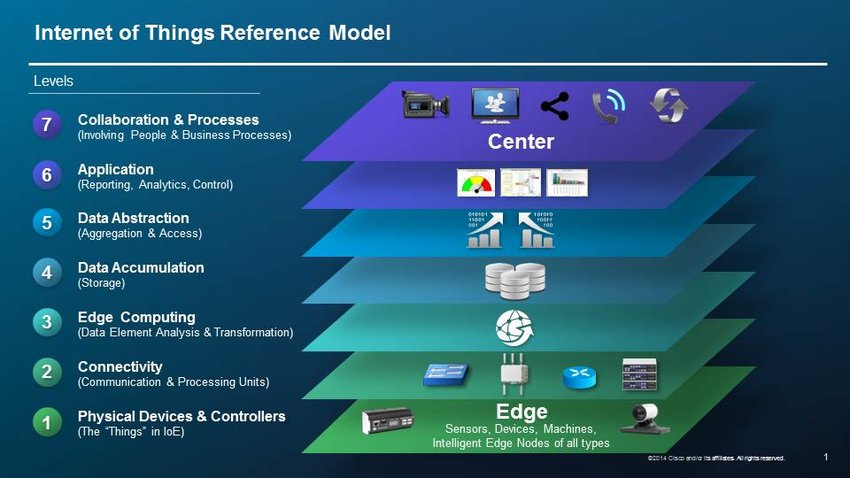
\includegraphics[width=\textwidth ]{img/Illustration-of-the-IoT-Reference-Model-by-Cisco-1.png}
	\caption{Архитектура интернета вещей, предложенная Cisco.}
	\label{fig:architecture}
\end{figure} 

\begin{enumerate}
	\item[1.] \textbf{Физические устройства и контроллеры} --- это уровень, содержащий вещи в IoT. Сюда входит широкий спектр конечных устройств, которые могут отправлять или получать информацию (например, датчики и считыватели радиочастотной идентификации (RFID)).
	\item[2.] \textbf{Соединение} --- это уровень, содержащий все компоненты, способные передавать информацию. Передача может осуществляться между устройствами на первом уровне, между компонентами на этом уровне или между первым и третьим уровнем.
	\item[3.] \textbf{Граничные (туманные) вычисления} (с английского Edge (Fog) computing) --- это первый уровень, на котором происходит обработка данных. Здесь могут собираться и предварительно обрабатываться значительные объёмы информации до того, как они будут переданы в верхние уровни. Данный уровень также позволяет форматировать и декодировать данные до того, как они будут обработаны. % Это может снизить нагрузку на более высокие уровни. 
	\item[4.] \textbf{Накопление данных} --- это уровень, на котором данные сохраняются, чтобы приложения могли получить к ним доступ в случае необходимости. Как правило, необходимая обработка информации не может быть выполнена на сетевых скоростях, поэтому вычислительная система нуждается в промежуточном хранилище данных. Сохранённые данные также могут быть преобразованы и рекомбинированы, чтобы быть готовыми к использованию на более высоких уровнях. В результате на этом уровне данные в движении преобразуются в данные в состоянии покоя.
	\item[5.] \textbf{Абстракция данных} --- это уровень, позволяющий хранить данные более эффективным образом для повышения производительности более высоких уровней. На данном уровне над данными могут выполняться операции нормализации, индексирования, форматирования, проверки, консолидации, а также обеспечивается доступ к нескольким хранилищам данных.
	\item[6.] \textbf{Приложения} --- это уровень, на котором информация, накопленная ранее, интерпретируется приложениями. Именно на этом уровне располагается бизнес-логика приложений.
	\item[7.] \textbf{Взаимодействие и процессы} --- это уровень, объединяющий всё вместе. Система бесполезна, если информация, предоставляемая на этом уровне, не является полезной. Данные из интернета вещей должны использоваться для принятия обоснованных решений.
\end{enumerate}

Операционные системы для интернета вещей принципиально меняют процесс разработки програмного обеспечения для систем с многоуровневой архитектурой, описанной выше, так как позволяют разработчикам абстрагироваться от особенностей аппаратуры конкретных устройств и предоставляют шаблоны для создания приложений с определённой архитектурой.

% Интернет Вещей --- это новая концепция, в которой Интернет эволюционирует от объединения компьютеров и людей к объединению умных вещей.

% Базовой идеей IoT является предоставление возможности автономного обмена полезной информацией между уникально идентифицируемыми объектами реального мира. Эти устройства оснащены новейшими технологиями, такими, как радиочастотная идентификация (RFID) и беспроводные сети датчиков (WSNs), и в дальнейшем получают возможность принимать самостоятельные решения в зависимости от того, какое автоматизированное действие выполняется. 

% Тем не менее, у разных людей и организаций есть свои отличающиеся концепции Интернета Вещей.

% 6-УРОВНЕВАЯ АРХИТЕКТУРА IOT

% Операционные системы устройств интернета вещей (ОСИВ, англ. Internet of Things Operating Systems, IoT OS) позволяют оснащать умные устройства, подключенные к интернету или иной сети связи, основными функциями компьютера с учётом ограниченности вычислительных ресурсов и специфических технических особенностей экосистемы интернета вещей. Такие ОС близки к ранее существовавшему классу операционных систем реального времени (ОСРВ, англ. RTOS)



\section{Сферы применения интернета вещей}

Чтобы поставить проблему выбора операционной системы для интернета вещей, необходимо обозначить круг задач, решаемых устройствами. Концепция интернета вещей находит своё применение во множестве различных сфер жизнедеятельности человека: как в быту, так и в промышленности. Далее будут рассмотрены сферы, в которых применяются IoT-системы, и обозначены задачи, которые ставятся перед умными устройствами.

\subsection{Интернет вещей в быту}

В быту интернет вещей применяется при проектировании умных домов. Системы интернета вещей способны автоматизировать бытовые процессы и исключить непосредственное участие человека. К таким процессам можно отнести дистанционное управление бытовой техникой, музыкальными системами и системами освещения. Автоматизация может выполняться при помощи сбора и анализа статистики о бытовых процессах. Принципы функционирования IoT, описанные на примере бытовых процессов, можно перенести на бесконечное множество любых других, начиная от уличного освещения и управления светофорами, и до управления огромными предприятиями и городами \cite{Kaspersky}.

\subsection{Промышленный интернет вещей}

Промышленный Интернет вещей (Industrial IoT, IIoT) \cite{Oracle} относится к применению технологии Интернета вещей в промышленных условиях. В последнее время в промышленности используется межмашинное взаимодействие (M2M) для обеспечения беспроводной автоматизации и управления. Но с появлением облачных и смежных технологий (таких как аналитика и машинное обучение) отрасли могут достичь нового уровня автоматизации и тем самым создать новые модели доходов и бизнеса. Организации, которые лучше всего подходят для IoT, --- это те, которые могут выиграть от использования умных устройств в своих бизнес-процессах. Ниже приведены некоторые распространенные варианты использования IIoT.

\subsubsection{Умные города}

В умных городах используются такие устройства интернета вещей, как датчики и счетчики для сбора и анализа данных. Полученные данные могут использоваться для улучшения инфраструктуры, коммунального обслуживания и других городских сервисов.

\subsubsection{Производства}

Производители могут получить конкурентное преимущество, используя мониторинг производственных линий, чтобы обеспечить упреждающее обслуживание оборудования с помощью датчиков, обнаруживающих надвигающийся сбой. С помощью оповещений от датчиков производители могут быстро проверять оборудование и ремонтировать его в случае необходимости. Это позволяет компаниям сократить эксплуатационные расходы, а также увеличить время безотказной работы и повысить эффективность оборудования.

\subsubsection{Транспорт и логистика}

Транспортные и логистические системы могут извлекать выгоду из приложений IoT, отслеживая параметры перевозимых грузов. Например, можно отслеживать температуру перевозимых продуктов питания и напитков, цветочной и фармацевтической продукции, чтобы отправлять предупреждения, когда температура поднимается или падает до уровня, угрожающего качеству товаров.
	
\subsubsection{Розничная торговля}

Приложения IoT позволяют розничным компаниям управлять запасами, улучшать качество обслуживания клиентов, оптимизировать цепочку поставок и сокращать эксплуатационные расходы.

\subsubsection{Государственный сектор}

Преимущества IoT в государственном секторе и других средах, связанных с услугами, достаточно обширны. Например, государственные коммунальные службы могут использовать приложения на базе интернета вещей для уведомления своих пользователей об отключениях и небольших перебоях в подаче воды и электроэнергии. Приложения IoT могут собирать данные о масштабах сбоев и управлять ресурсами, чтобы помогать коммунальным службам быстрее восстанавливать работу после сбоев.

\subsubsection{Здравоохранение}

Интернет вещей является важным аспектом \textit{телемедицины} \cite{Kaspersky} (для обозначения интернета медицинских вещей иногда используется аббревиатура IoMT). Примеры его применения включают удаленную медицинскую диагностику, цифровую передачу медицинских изображений, видеоконсультации со специалистами и прочее. Приложения IoT также используются в носимых устройствах, которые могут контролировать здоровье человека и условия окружающей среды. Такие приложения не только помогают людям следить за состоянием своего здоровья, но и позволяют врачам удаленно наблюдать за пациентами.

\subsubsection{Общая безопасность во всех отраслях}

Помимо отслеживания физических показателей, IoT можно использовать для повышения безопасности труда. Сотрудники опасных предприятий, таких как шахты, месторождения и электростанции, должны знать о возможном наступлении опасной ситуации. Когда они подключены к приложениям на основе датчиков IoT, они могут быть уведомлены об авариях, чтобы предпринять необходимые действия.



\section{Проблема выбора операционной системы для интернета вещей}

Операционные системы, предназначенные для интернета вещей, обладают различной функциональностью, которая определяет преимущества и недостатки каждого конкретного решения. Выбранная операционная система должна полностью соответствовать требованиям и ограничениям, предъявляемым к устройствам. Можно выделить четыре основных аспекта и перечень главных вопросов, которые разработчики устройств учитывают при выборе ОС для периферийных устройств IoT \cite{OS_questions}.

% Перед принятием окончательного решения необходимо ответить на четыре основных вопроса.


\begin{enumerate}
	\item[1.] \textbf{Какой уровень надежности и долгосрочной поддержки необходим?} \newline 
	Под надёжностью в данном случае понимается соответствие операционной системы определенным стандартам и сертификациям. Необходимо, чтобы выбранная операционная система обеспечивала варианты, подходящие для конкретных отраслевых стандартов и требований.
	\item[2.] \textbf{Какие требования предъявляются к производительности?} \newline 
	Выбранная операционная система должна соответствовать требованиям устройства к вычислительной мощности и производительности в реальном времени. Также при ответе на данный вопрос стоит учитывать другие аспекты, связанные с производительностью и оказывающие влияние на выбор ОС. К таким можно отнести энергопотребление и объём памяти устройства, а также требования к времени отклика системы на внешние события.
	\item[3.] \textbf{Обеспечивает ли операционная система безопасность устройства?} \newline 
	Безопасность --- один из основных факторов, учитываемых при разработке устройств интернета вещей. Это касается и используемой ОС, так как от неё зависит целостность данных, собираемых устройствами. Если система не обеспечивает необходимый уровень безопасности, то это может привести к порче или краже данных, нарушению запланированных процессов.
	\item[4.] \textbf{Является ли выбранная операционная система масштабируемой?} \newline 
	В связи с тем, что операционные системы, как и любое программное обеспечение, меняются вместе с требованиями к функциям, которые они должны предоставлять. Разработка IoT-устройства с масштабируемой ОС позволяет в будущем адаптироваться к другим задачам без внесения значительных изменений. Масштабируемые ОС могут обрабатывать дополнительные ресурсы без изменения скорости вывода, охватывать несколько устройств и географических регионов.
\end{enumerate}

% Для объединения умных вещей в информационные сети необходимо соответствующее программное обеспечение. Ввиду его сложности ...

% Операционная система - это основная программа IoT-проекта. Современная операционная система Интернета вещей использует технологию облачных вычислений для управления устройствами Интернета вещей в любой точке мира. Благодаря небольшому объему памяти и более высокой эффективности каждая операционная система, представленная ниже, может удовлетворить требования пользователя.




%%% Local Variables:
%%% mode: latex
%%% TeX-master: "rpz"
%%% End:

\chapter{Описание существующих решений}
\label{cha:methods}

В данном разделе будет проведён анализ существующих операционных систем для устройств интернета вещей. Рассматриваемые операционные системы будут относиться к одному из двух типов: ОС реального времени и ОС разделения времени.

Стараться указывать тип ядра ОС, а также информацию по остальным критериям сравнения.

\section{Операционные системы реального времени}

\subsection{Azure RTOS}

\cite{OS_questions}



\subsection{(Amazon) FreeRTOS}



\subsection{Zephyr}



\subsection{ОСРВ МАКС}



\section{Операционные системы разделения времени}



\subsection{Windows 10 IoT}

3 версии: Windows 10 IoT Core, Windows 10 IoT Enterprise и Windows IoT Server. \cite{OS_questions}



\subsection{Azure Sphere}

\cite{OS_questions}



\subsection{Azure IoT Edge}

\cite{OS_questions}



\subsection{Azure Sphere}

\cite{OS_questions}



\subsection{Contiki}



\subsection{Mbed OS}



\subsection{Android Things}



\subsection{Huawei LightOS}



\subsection{TinyOS}



\subsection{Ubuntu Core}

Snappy - OS with Ubuntu Core?


\subsection{Raspbian}

Вроде бы сделана только для Raspberry Py, то есть непереносимая.



\subsection{RIOT}



\subsection{Fuchsia OS}



Если этого мало, то здесь (https://www.intuz.com/top-iot-operating-systems-for-iot-devices) есть ещё больше.



%%% Local Variables:

%%% mode: latex
%%% TeX-master: "rpz"
%%% End:
\chapter{Классификация существующих решений}
\label{cha:classification}

В данном разделе будут описаны критерии сравнения операционных систем для устройств интернета вещей

\section{Критерии сравнения операционных систем}

Описание (и желательно обоснование) критериев сравнения.

Критерии:

\begin{itemize}
	\item Тип ядра: монолитное или микроядро;
	\item Тип лицензии;
	\item Поддержка POSIX;
	\item Тип многозадачности: вытесняющая, кооперативная, отсутствует;
	\item Кроссплатформенность или переносимость (бинарный признак);
	\item ????? Открытый/закрытый исходный код;
	\item ????? Поддержка SMP;
	\item ????? Популярность (востребованность) на рынке (мб взять статистику популярности ОС и сравнивать по объёму доли на рынке в \%);
	\item ????? Промышленное применение (бинарный признак, типа может быть только промышленное и частное применение).
\end{itemize}

Наличие сетевых функций не оценивается, так как все ОС, рассматриваемые в данной работе, являются сетевыми.

\section{Сравнительный анализ операционных систем}

Сводная таблица сравнения операционных систем. \newline

Если по всем критериям одна из систем оказывается лучшей из описываемых, то задать себе закономерный вопрос, почему остальные системы ещё используются. Предложить ещё один критерий сравнения.



\backmatter %% Здесь заканчивается нумерованная часть документа и начинаются ссылки и
            %% заключение

\section*{Заключение}
\addcontentsline{toc}{section}{Заключение}

В рамках научно-исследовательской работы была проведена классификация сетевых операционных систем для устройств интернета вещей.

В результате сравнения были выделены: 

\begin{itemize}
	\item Azure Sphere, Windows 10 IoT и Amazon FreeRTOS как наиболее функциональные и масштабируемые;
	\item ОСРВ МАКС и KasperskyOS как наиболее доступные с точки зрения использования прикладных служб;
	\item Ubuntu Core и Raspbian как наиболее адаптированные для бытового применения.
\end{itemize}

В ходе выполнения данной работы были решены следующие задачи.

\begin{enumerate}[label*=\arabic*.]
\item Проведён анализ предметной области интернета вещей;
\item Рассмотрены существующие операционные системы для устройств интернета вещей;
\item Сформулированы критерии сравнения и оценки рассмотренных операционных систем;
\item Проведён сравнительный анализ существующих решений по выделенным критериям. 
\end{enumerate}

Таким образом, все поставленные задачи были выполнены, поставленная цель достигнута.

\pagebreak

% % Список литературы при помощи BibTeX
% Юзать так:
%
% pdflatex rpz
% bibtex rpz
% pdflatex rpz

\bibliographystyle{ugost2008}
\bibliography{rpz}


%%% Local Variables: 
%%% mode: latex
%%% TeX-master: "rpz"
%%% End: 


% \appendix   % Тут идут приложения

% \include{90-appendix1}
% \include{91-appendix2}
% \include{92-appendix3}
% \include{93-appendix4}

\end{document}

%%% Local Variables:
%%% mode: latex
%%% TeX-master: t
%%% End:
